% Uses Springer LNCS format for ICTAC 2026 submission
\documentclass[runningheads]{llncs}
\usepackage{graphicx}
\usepackage{amsmath}
\usepackage{amssymb}
\usepackage{booktabs}
\usepackage{subcaption}
\usepackage{tikz}
\usetikzlibrary{arrows.meta,positioning,shapes.geometric}
\usepackage{hyperref}
\usepackage{microtype}

% Bold run-in \paragraph headings (llncs defaults to italic)
\makeatletter
\renewcommand\paragraph{\@startsection{paragraph}{4}{\z@}%
                       {-12\p@ \@plus -4\p@ \@minus -4\p@}%
                       {-0.5em \@plus -0.22em \@minus -0.1em}%
                       {\normalfont\normalsize\bfseries}}
\makeatother

\title{Tool Support for Causal Reasoning \\ via String Diagram Surgery}
\titlerunning{Tool Support for Causal Reasoning via String Diagram Surgery}

\author{Sifei Li and Fabio Zanasi}
\institute{University College London, United Kingdom}

\begin{document}
\maketitle

\begin{abstract}
Causal inference and counterfactual reasoning have recently been given a category-theoretic semantics based on string diagrams and their graphical manipulation (``surgery''). Despite these theoretical advances, there is currently no software support for this approach. In this work, we present a prototype implementation in Julia that enables causal and counterfactual queries to be evaluated on probabilistic models represented as string diagrams. This allows us to compare the categorical approach, both conceptually and empirically, with existing implementations in R and Python. In particular, we show that the use of an explicit diagrammatic intermediate representation can achieve competitive performance while offering greater structural transparency and interpretability.
\end{abstract}

%The submission is intended as an ICTAC 2026 tool paper: the prototype implementation contains a concrete artifact in \texttt{src/} and \texttt{tools/}, a documented pipeline, and empirical evidence that shows the value of categorical diagrammatic representations for practical causal inference.


\section{Introduction}
Causal inference studies how actions and interventions change the behaviour of complex systems \cite{pearl2009causality}, answering questions such as ``what is the effect of a drug on recovery?'' that purely statistical association cannot. Central to it is the problem of \emph{identification}: given a causal model and available data, can a target interventional or counterfactual query be uniquely expressed in terms of observable quantities? Under hidden confounding this becomes non-trivial; the classic ID algorithm and its counterfactual extension ID-CF \cite{shpitser2008complete} characterise when identification is possible.

Counterfactuals are an especially expressive class: they ask what would have happened under an alternate intervention, often conditioned on observed evidence. A typical query $P(Y_{x}=y \mid X=x', Z=z)$ asks how the outcome would change if $X$ were set to $x$ when in fact $X=x'$ was observed. Grounded in Pearl's counterfactual semantics \cite{pearl2009causality}, such questions are central to explanation, responsibility attribution, policy evaluation, and fairness.

Recent work, initiated by~\cite{jacobs2019causal} and further developed in \cite{jacobs2021causal,lorenz2023causal,tull2023activeinference,friend2025compositional}, has shown that causal inference can be given a rigorous compositional semantics using category theory, most notably the theory of \emph{Markov categories}~\cite{fritz2020synthetic,jacobs2015} and of \emph{string diagrams}~\cite{intro_to_string_diagram}. In this perspective, a Bayesian network is not merely a graph, but a morphism in a symmetric monoidal category, represented graphically as a string diagram where wires indicate variables and boxes indicate conditional mechanisms. Interventions are then modelled as local rewrites of these diagrams (`surgeries'~\cite{jacobs2019causal}), and counterfactual constructions~\cite{jacobs2021causal} correspond to pairs of string diagrams that share latent sources.

The advantage of this semantics is that it makes structural causal reasoning explicit: rather than manipulating symbolic formulas alone, one works with compositional diagrams whose topology encodes causal constraints, and surgery exposes the local structure of interventions and confounding. It is attractive for tool support in particular, since the same diagrammatic primitives are re-used across model construction, intervention, and simplification.

Despite the growing theoretical prominence of string diagram surgery, there is not yet a single system that implements counterfactual identification directly on this semantics. Existing projects provide complementary functionality — categorical probabilistic libraries~\cite{cho2017efprob}, quantum circuit tooling~\cite{kissinger2024pqs}, and general string-diagram manipulators (e.g.~\cite{caldwell2026tensorrocq,chyp2024}) — but a focused pipeline for diagrammatic counterfactual identification is still missing. In this work we take the first steps to address this gap. Our contributions are:
\begin{itemize}
    \item We present an implementation of counterfactual identification based on string diagram surgery, realised in Julia with the Catlab ecosystem.
    \item We analyse the concrete challenges of implementing categorical causal semantics, including diagram representation, parallel world construction, and simplification.
    \item We connect the implementation to the broader string diagrammatic reasoning ecosystem through Chyp export, and outline how the same infrastructure can extend toward richer probabilistic semantics.
    \item We compare our implementation with existing R and Python alternatives, identifying the cases where a categorical approach performs better or worse and clarifying the trade-offs involved.
\end{itemize}

%The remainder of the paper is organised as follows. Section~\ref{sec:background} reviews the categorical background and string diagram view of Bayesian networks. Section~\ref{sec:implementation} describes the implementation choices and available functionality. Section~\ref{sec:discussion} compares the tool with existing work and highlights experimental evidence. Section~\ref{sec:conclusion} concludes.

\section{Categorical Background}\label{sec:background}

We recall just enough of the diagrammatic semantics of causal models to phrase the three kinds of query our tool answers. Throughout we follow the string-diagram approach to causality of Jacobs, Kissinger and Zanasi~\cite{jacobs2021causal,jacobs2019causal}, introducing each notion on a single running example---a commuter's daily journey---and keeping the category theory to the minimum needed to read the diagrams.

\begin{figure}[t]
\centering
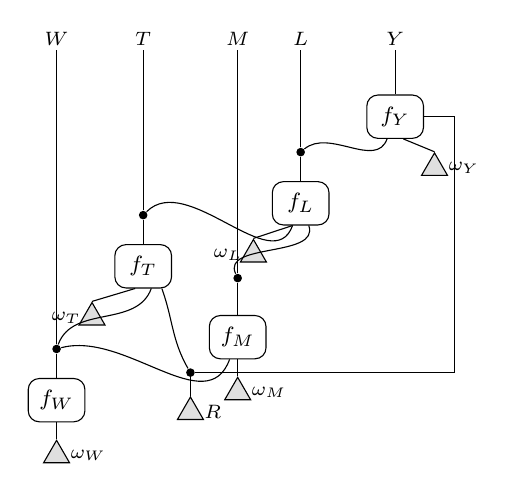
\begin{tikzpicture}[>=Stealth, font=\footnotesize,
  box/.style={draw, rounded corners, fill=white, minimum width=0.72cm, minimum height=0.55cm, inner sep=1pt},
  st/.style={fill=gray!25, draw, regular polygon, regular polygon sides=3, inner sep=0pt, minimum size=3.8mm},
  cp/.style={circle, fill, inner sep=1.1pt},
  wl/.style={inner sep=1.5pt, font=\scriptsize}
]
% mechanisms (read bottom to top)
\node[box] (fW) at (0.0,0.7) {$f_W$};
\node[box] (fT) at (1.1,2.4) {$f_T$};
\node[box] (fM) at (2.3,1.5) {$f_M$};
\node[box] (fL) at (3.1,3.2) {$f_L$};
\node[box] (fY) at (4.3,4.3) {$f_Y$};
% states (noise + latent), apex up
\node[st] (wW) at (0.0,0.0) {}; \node[wl,right=0pt of wW]{$\omega_W$};
\node[st] (wT) at (0.45,1.75){};\node[wl,left=-1pt of wT]{$\omega_T$};
\node[st] (wM) at (2.3,0.8) {}; \node[wl,right=0pt of wM]{$\omega_M$};
\node[st] (wL) at (2.5,2.55){}; \node[wl,left=-1pt of wL]{$\omega_L$};
\node[st] (wY) at (4.8,3.65){}; \node[wl,right=0pt of wY]{$\omega_Y$};
\node[st] (R)  at (1.7,0.55){}; \node[wl,right=0pt of R]{$R$};
% copy dots
\node[cp] (cW) at (0.0,1.35){};
\node[cp] (cR) at (1.7,1.05){};
\node[cp] (cT) at (1.1,3.05){};
\node[cp] (cM) at (2.3,2.25){};
\node[cp] (cL) at (3.1,3.85){};
% noise into mechanisms (from below)
\draw (wW.north) -- (fW.south);
\draw (wT.north) -- (fT.250);
\draw (wM.north) -- (fM.south);
\draw (wL.north) -- (fL.250);
\draw (wY.north) -- (fY.290);
% W copied to output, f_T, f_M
\draw (fW.north) -- (cW);
\draw (cW) -- (0.0,5.15) node[wl,above]{$W$};
\draw (cW) to[out=70,in=250] (fT.290);
\draw (cW) to[out=15,in=250] (fM.250);
% R copied to f_T and (up the right margin) f_Y
\draw (R.north) -- (cR);
\draw (cR) to[out=120,in=290] (fT.310);
\draw (cR) -- (5.05,1.05) -- (5.05,4.3) -- (fY.east);
% T copied to output and f_L
\draw (fT.north) -- (cT);
\draw (cT) -- (1.1,5.15) node[wl,above]{$T$};
\draw (cT) to[out=45,in=250] (fL.250);
% M copied to output and f_L
\draw (fM.north) -- (cM);
\draw (cM) -- (2.3,5.15) node[wl,above]{$M$};
\draw (cM) to[out=115,in=290] (fL.290);
% L copied to output and f_Y
\draw (fL.north) -- (cL);
\draw (cL) -- (3.1,5.15) node[wl,above]{$L$};
\draw (cL) to[out=40,in=250] (fY.250);
% Y output
\draw (fY.north) -- (4.3,5.15) node[wl,above]{$Y$};
\end{tikzpicture}
\caption{The commute model as a string diagram, read bottom to top. Each box is a \emph{mechanism} $f_X$ taking its parents and a private noise state $\omega_X$ (triangles) to the variable $X$; black dots \emph{copy} a value to several consumers, exposing each variable as an output wire at the top. The confounding $T\leftrightarrow Y$ is the shared latent state $R$ copied into both $f_T$ and $f_Y$. The whole diagram denotes the joint distribution over $W,T,M,L,Y$.}
\label{fig:bn-string}
\end{figure}

\paragraph{Bayesian Networks as String Diagrams.}
Figure~\ref{fig:bn-string} renders our running \emph{commute} model as a string diagram (read bottom to top). The model has five observable variables: weather $W$, departure time $T$, mode of transport $M$, lateness $L$, and work performance $Y$. They label the wires in the diagram.To each variable $X$ is associated a \emph{mechanism} $f_X \colon \Big(\textstyle\bigotimes_{V \in \mathrm{pa}(X)} V\Big)\otimes \Omega_X \;\longrightarrow\; X$, depicted as a box: its meaning is a function that reads the variables that are its direct causes (its parents $\mathrm{pa}(X)$) together with a private noise source $\omega_X$---an exogenous state modelling everything left unmodelled, depicted as a triangle---and outputs a probability distribution over $X$. At a glance, the representation of this model as a string diagram resembles a Bayesian network. However, unlike networks, string diagrams are \emph{algebraic} entities: understood as morphisms of a symmetric monoidal category (SMC), they can be reasoned about compositionally through that monoidal structure. Within this perspective, we interpret each box as a morphism of an SMC, and the whole string diagram results from assembling them together by sequential composition and monoidal product (depicted as vertical and horizontal juxtaposition respectively). Variables are the objects of the SMC, and states are morphisms with no input. For each object we assume a \emph{copy} map (black dots) that duplicate a value, and a \emph{discard} map that delete it. A category equipped with these compatibly is a \emph{copy--discard} (or Markov) category~\cite{fritz2020synthetic,jacobs2015}, which constitutes a basic algebraic framework for probabilistic computation. In our example, a copy dot is inserted wherever a variable feeds several mechanisms, so that the same value can be both passed on and exposed as an observed output. \emph{Confounding}---a hidden common cause of two variables, which we write $T\leftrightarrow Y$---is represented diagrammatically by a single latent state $R$ copied into both $f_T$ and $f_Y$ (Figure~\ref{fig:bn-string}): for the commuter, an unobserved factor (say, a recurring engineering work pattern) influences both when she sets off and how she ultimately performs.


%Composing all five mechanisms yields one diagram whose denotation is the joint distribution over $W,T,M,L,Y$. Routing every source of randomness through the explicit noise states $\omega_X$ leaves the mechanisms themselves \emph{deterministic}: a small move that pays off below, since two scenarios can then be made to share exactly the same randomness.


\paragraph{Interventions by Surgery.}
To ask what happens if we \emph{force} a variable to a value---Pearl's $\mathrm{do}(T{=}t)$---we perform \emph{string diagram surgery}~\cite{jacobs2021causal,jacobs2019causal,lorenz2023causal}: we cut the wires entering the mechanism $f_T$, discarding its parents and noise, and replace $f_T$ by a \emph{sharp state} $\mathsf{do}(T{=}t):I\to T$, the deterministic distribution concentrated at $t$. Graphically $T$ is severed from its causes while the rest of the diagram is left untouched, so the surgered diagram denotes the interventional distribution $P(\,\cdot\mid\mathrm{do}(T{=}t))$. Surgery is thus a purely \emph{local} rewrite, in contrast with the global symbolic substitutions of the algebraic account; this locality is what makes it amenable to mechanical manipulation.

\paragraph{Example 1: A Counterfactual Query.}
Counterfactuals compare what happened with what \emph{would have} happened. For the commuter we ask: \emph{given that she actually left at time $t'$ and would have taken mode $m$ under the prevailing weather, what would her performance $Y$ have been had she instead left at time $t$?}---a query of the form $P(Y_t \mid T{=}t',\,M{=}m)$. The factual and the hypothetical are different worlds, yet they concern the same commuter and so share the same hidden causes. We represent this by a \emph{twin}, or parallel-world, diagram~\cite{jacobs2021causal}: two copies of the model, with surgery applied only in the world where $T$ is set to $t$, and the latent state $R$ \emph{copied into both worlds} so they stay coupled through their common randomness (Figure~\ref{fig:re-pw}). Here the deterministic mechanisms matter: sharing $R$ shares the actual circumstances across worlds. Factual observations ($T{=}t'$, $M{=}m$) are imposed by attaching \emph{sharp effects}---the duals of sharp states---to the corresponding output wires.

\paragraph{Example 2: A Causal-Inference Query by Comb Disintegration.}
Often we want a plain interventional effect such as $P(Y\mid\mathrm{do}(T))$, but the confounder $T\leftrightarrow Y$ blocks reading it directly off the observational distribution. The diagrammatic remedy is \emph{comb disintegration}~\cite{jacobs2021causal}. A \emph{comb} is a process with a hole---drawn as a box with a rectangular bite removed---into which another process can be plugged; it is the diagrammatic shape of a conditional that still awaits one of its inputs. One factors the observable part of the model as a comb $g$ whose hole sits exactly where the confounded mechanism would go, leaving a process $f$ as its filler, so that plugging $f$ into $g$ recovers the joint distribution:
\begin{center}
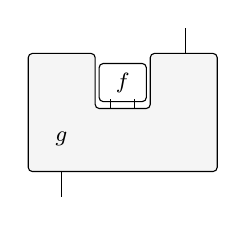
\begin{tikzpicture}[>=Stealth, font=\footnotesize, baseline,
  bx/.style={draw, rounded corners=1.5pt, fill=white}]
% comb g: a box with a rectangular bite out of its top edge
\draw[rounded corners=1.5pt, fill=gray!8]
  (0,0) -- (2.4,0) -- (2.4,1.5) -- (1.55,1.5) -- (1.55,0.8)
  -- (0.85,0.8) -- (0.85,1.5) -- (0,1.5) -- cycle;
\node at (0.42,0.42) {$g$};
% filler f plugged into the hole
\node[bx, minimum width=0.6cm, minimum height=0.42cm] (f) at (1.2,1.13) {$f$};
\draw (1.05,0.92) -- (1.05,0.8);
\draw (1.35,0.92) -- (1.35,0.8);
% external input (bottom) and output (top)
\draw (0.42,0) -- (0.42,-0.32);
\draw (2.0,1.5) -- (2.0,1.82);
\end{tikzpicture}
\end{center}
\emph{Disintegrating} the observed joint re-expresses $f$ in terms of observable conditionals; plugging the surgically modified $f$ back into $g$ then yields $P(Y\mid\mathrm{do}(T))$ as a formula over observable quantities. The classical back- and front-door adjustments are special cases, and this is precisely the procedure realised by the comb-based causal-inference extension of Section~\ref{sec:implementation}.

\paragraph{Identifiability.}
A query is \emph{identifiable} when it can be rewritten purely in terms of the observational distribution. After surgery and simplification the diagram splits into maximal confounded blocks---its \emph{c-components} (or districts)---whose diagrammatic counterparts are the \emph{R-fragments} the implementation extracts and rewrites. Identification succeeds exactly when every fragment's exogenous noise can be absorbed into a consistent observable expression; for counterfactuals this decision is made by the ID-CF algorithm~\cite{shpitser2008complete}, whose diagrammatic realisation is the subject of the next section.

\section{Implementation}\label{sec:implementation}

We implemented the approach in Julia on top of the Catlab ecosystem~\cite{catlab}, which realises symmetric monoidal categories through \emph{wiring diagrams}, the concrete data structure for a string diagram. The whole computation manipulates a single such \texttt{WiringDiagram}, in which boxes are mechanisms (morphisms) and wires variable dependencies. Each box carries a symbolic name encoding its role---\texttt{f\_X} for a mechanism, \texttt{PU\_X} for an exogenous source, \texttt{do\_X=x} for an intervention (a \emph{sharp state}), \texttt{obs\_X=x} for an observation (a \emph{sharp effect}), \texttt{c\_X} for a deterministic constant mechanism---so that surgery and identification are uniformly rewrites on named boxes and their wiring.

\paragraph{Pipeline, Illustrated on a Worked Example.}
We follow a single \emph{commute} scenario through the entire pipeline. The model has variables \(W,T,M,L,Y\)---weather, departure time, mode of transport, lateness, and final work performance---and the counterfactual query asks: for someone who actually left at time \(t'\) under weather \(w\), what would their work performance have been if they had left at time \(t\), given the additional behavioural evidence that, under the same weather, they would use transport mode \(m\)? Identification is driven by a single entry point, \texttt{identify\_counterfactual} (alias \texttt{run\_cf\_pipeline}) in \texttt{src/id\_cf.jl}, which executes five stages, timing each independently and exporting an intermediate diagram after every stage (dashed arrows below mark the Chyp trace). Figure~\ref{fig:running-example} carries the commute model through all five:

\begin{center}
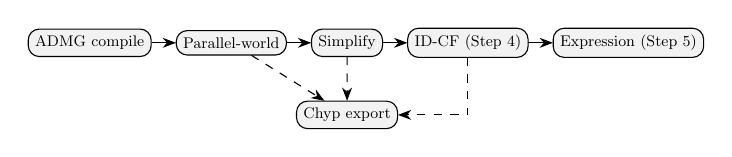
\begin{tikzpicture}[>=Stealth, scale=0.62, transform shape, node distance=0.5cm, every node/.style={font=\small, draw, rectangle, rounded corners, fill=gray!10, inner sep=4pt}]
\node (admg) {ADMG compile};
\node[right=of admg] (parallel) {Parallel-world};
\node[right=of parallel] (simp) {Simplify};
\node[right=of simp] (idf) {ID-CF (Step~4)};
\node[right=of idf] (output) {Expression (Step~5)};
\node[below=0.9cm of simp] (chyp) {Chyp export};
\draw[->] (admg) -- (parallel);
\draw[->] (parallel) -- (simp);
\draw[->] (simp) -- (idf);
\draw[->] (idf) -- (output);
\draw[->, dashed] (parallel) -- (chyp);
\draw[->, dashed] (simp) -- (chyp);
\draw[->, dashed] (idf.south) |- (chyp.east);
\end{tikzpicture}
\end{center}

\begin{enumerate}
    \item \textbf{ADMG compilation} (\texttt{src/admg\_compile.jl}). The input Acyclic Directed Mixed Graph (ADMG) is \emph{rootified}---each bidirected edge $X \leftrightarrow Y$ is replaced by a fresh latent root feeding both endpoints---and then compiled by \texttt{graph\_b\_to\_scm} into a base structural diagram with one mechanism box $f_V : (\mathrm{pa}(V), U_V) \to V$ and one exogenous source $PU_V$ (the noise state $\omega_V$ of Section~\ref{sec:background}) per variable. For the commute model the bidirected edge $T\leftrightarrow Y$ becomes a shared latent root $R$ feeding both $T$ and $Y$ (Figure~\ref{fig:re-admg}).
    \item \textbf{Parallel-world construction} (\texttt{src/build\_multiverse}). The base diagram is lifted into a multiverse diagram by duplicating each mechanism box once per world while \emph{sharing} the exogenous source boxes across all worlds---the diagrammatic counterpart of shared exogenous noise. An intervened variable splits into a discarded sink and a fresh \texttt{do\_X=x} source; an observed variable receives an \texttt{obs\_X=x} sharp-effect box. Here the factual outcome $Y$ and the counterfactual $Y_t$ remain coupled through the shared root $R$ (Figure~\ref{fig:re-pw}).
    \item \textbf{Simplification} (\texttt{src/simplify\_cf.jl}). Four rewrite passes reduce the diagram to canonical form: pruning discarded branches and dead boxes, separating sharp effects from copy/fan-out, merging deterministic mechanisms with identical input sources, and absorbing exogenous noise by replacing each $f_X$ with a deterministic constant mechanism $c_X$ (Figure~\ref{fig:re-simplified}).
    \item \textbf{ID-CF identification} (Step~4, \texttt{src/id\_cf.jl}). The simplified diagram is decomposed into \emph{R-fragments}---the diagrammatic counterpart of c-components (districts) in ADMGs---and each fragment is rewritten by case analysis into an interventional probability box $P(C_l, F_l^{out} \mid \mathrm{do}(D_l), \mathrm{do}(F_l^{in}))$. A residual unabsorbed exogenous source signals a non-identifiable query.
    \item \textbf{Expression output} (Step~5, \texttt{id\_cf\_step5}). The resulting probability boxes are parsed into a small expression tree and rendered as a LaTeX formula, with optional algebraic simplification (e.g.\ dropping vacuous interventions and eliminating normalised summations); the identified estimand for the commute query is shown in Figure~\ref{fig:re-expr}.
\end{enumerate}
Supporting modules---Bayesian-network import from \texttt{.bif}/\texttt{.net} files, Chyp serialisation~\cite{chyp2024} for inspection, and shared graph utilities---together with the command-line driver and the worked commute example, are mapped in the top-level \texttt{README.md}, which first-time users should open first: its quickstart runs this full pipeline and the comb-disintegration examples of the next paragraph.

\begin{figure}[!t]
\centering
\begin{subfigure}[b]{0.48\textwidth}
\centering
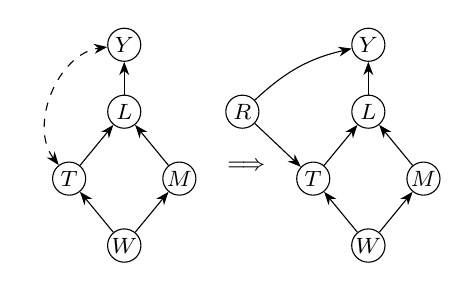
\begin{tikzpicture}[>=Stealth, font=\footnotesize,
   v/.style={circle, draw, inner sep=0.5pt, minimum size=4.2mm}]
\node[v] (W) at (0,0) {$W$};
\node[v] (T) at (-0.7,0.85) {$T$};
\node[v] (M) at (0.7,0.85) {$M$};
\node[v] (L) at (0,1.7) {$L$};
\node[v] (Y) at (0,2.55) {$Y$};
\draw[->] (W)--(T); \draw[->] (W)--(M);
\draw[->] (T)--(L); \draw[->] (M)--(L); \draw[->] (L)--(Y);
\draw[<->, dashed] (T) to[bend left=60] (Y);
\node at (1.55,1.0) {$\Longrightarrow$};
\begin{scope}[xshift=3.1cm]
\node[v] (W2) at (0,0) {$W$};
\node[v] (T2) at (-0.7,0.85) {$T$};
\node[v] (M2) at (0.7,0.85) {$M$};
\node[v] (L2) at (0,1.7) {$L$};
\node[v] (Y2) at (0,2.55) {$Y$};
\node[v] (R2) at (-1.6,1.7) {$R$};
\draw[->] (W2)--(T2); \draw[->] (W2)--(M2);
\draw[->] (T2)--(L2); \draw[->] (M2)--(L2); \draw[->] (L2)--(Y2);
\draw[->] (R2)--(T2); \draw[->] (R2) to[bend left=15] (Y2);
\end{scope}
\end{tikzpicture}
\caption{Input ADMG and its rootification ($T\leftrightarrow Y\Rightarrow R$).}
\label{fig:re-admg}
\end{subfigure}%
\hfill
\begin{subfigure}[b]{0.48\textwidth}
\centering
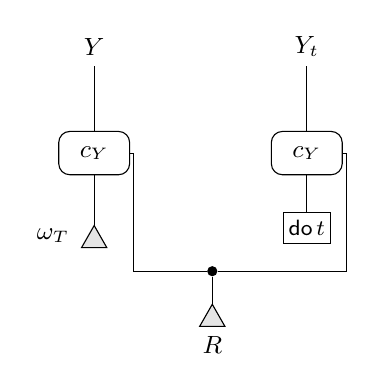
\begin{tikzpicture}[>=Stealth, font=\small,
  box/.style={draw, rounded corners, fill=white, minimum width=0.9cm, minimum height=0.55cm, inner sep=2pt},
  sb/.style={draw, fill=white, font=\footnotesize, inner sep=2pt, minimum height=0.4cm},
  cp/.style={circle, fill, inner sep=1.3pt}
]
% shared latent R at the bottom, apex up
\draw[fill=gray!20] (-0.16,-0.2) -- (0.16,-0.2) -- (0,0.08) -- cycle;
\node[below=0pt] at (0,-0.2) {$R$};
\node[cp] (cu) at (0,0.5) {};
\draw (0,0.08) -- (cu);
% factual world (left)
\node[box] (cy1) at (-1.5,2.0) {$c_Y$};
\draw[fill=gray!20] (-1.66,0.8) -- (-1.34,0.8) -- (-1.5,1.08) -- cycle;
\node[left=1pt] at (-1.66,0.95) {$\omega_T$};
\draw (cu) -- (-1.0,0.5) -- (-1.0,2.0) -- (cy1.east);
\draw (-1.5,1.08) -- (cy1.south);
\draw (cy1.north) -- (-1.5,3.1);
\node at (-1.5,3.35) {$Y$};
% counterfactual world (right)
\node[box] (cy2) at (1.2,2.0) {$c_Y$};
\node[sb] (dox) at (1.2,1.05) {$\mathsf{do}\,t$};
\draw (cu) -- (1.7,0.5) -- (1.7,2.0) -- (cy2.east);
\draw (dox.north) -- (cy2.south);
\draw (cy2.north) -- (1.2,3.1);
\node at (1.2,3.35) {$Y_t$};
\end{tikzpicture}
\caption{Parallel worlds: factual $Y$ and counterfactual $Y_t$ share the latent $R$.}
\label{fig:re-pw}
\end{subfigure}

\vspace{0.6em}

\begin{subfigure}[b]{0.48\textwidth}
\centering
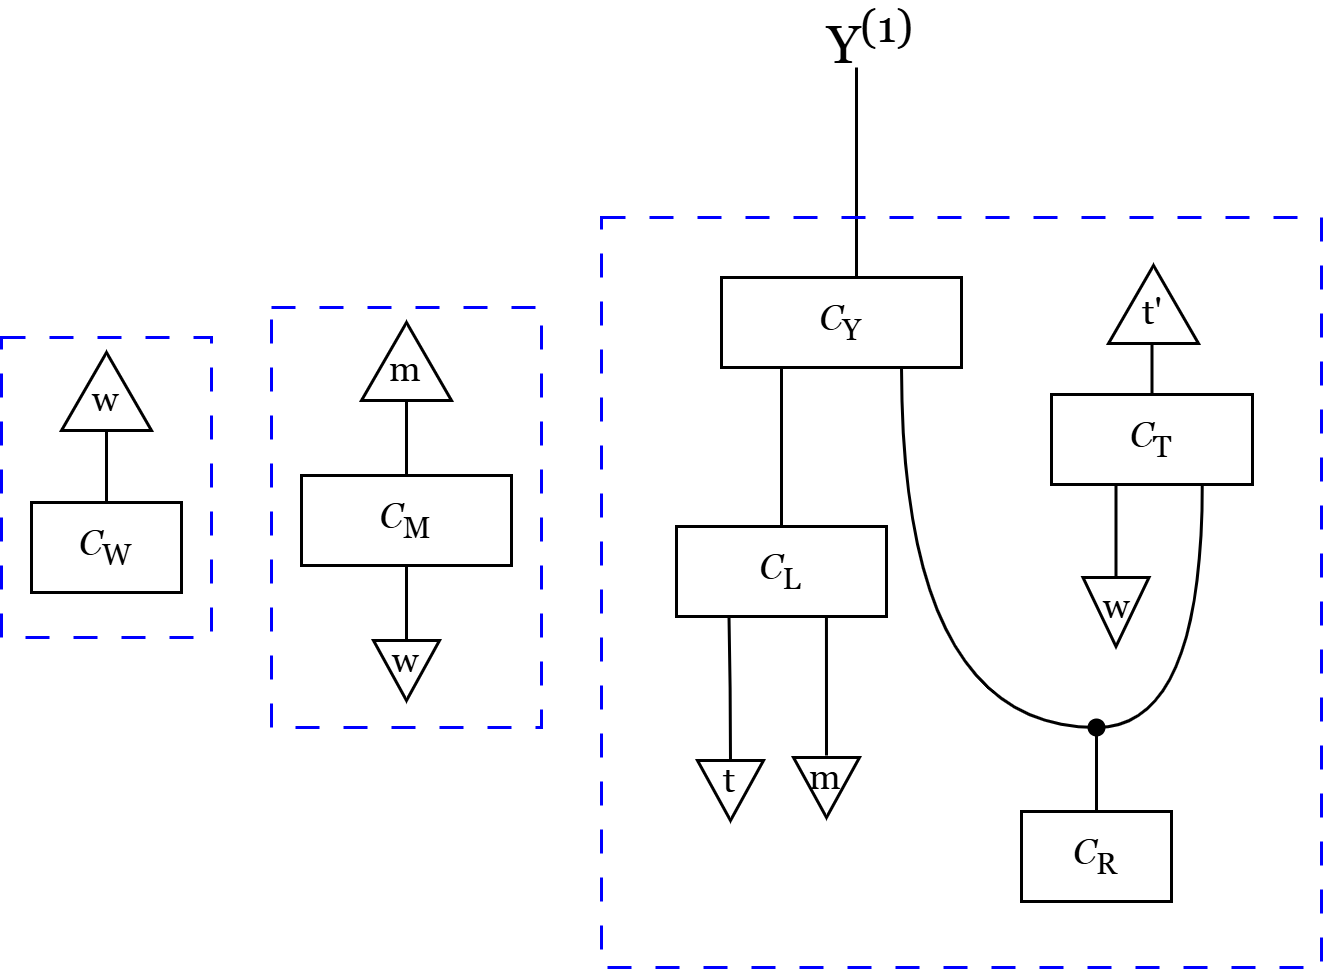
\includegraphics[width=\textwidth]{simplify.png}
\caption{Simplified string diagram.}
\label{fig:re-simplified}
\end{subfigure}
\hfill
\begin{subfigure}[b]{0.48\textwidth}
\centering
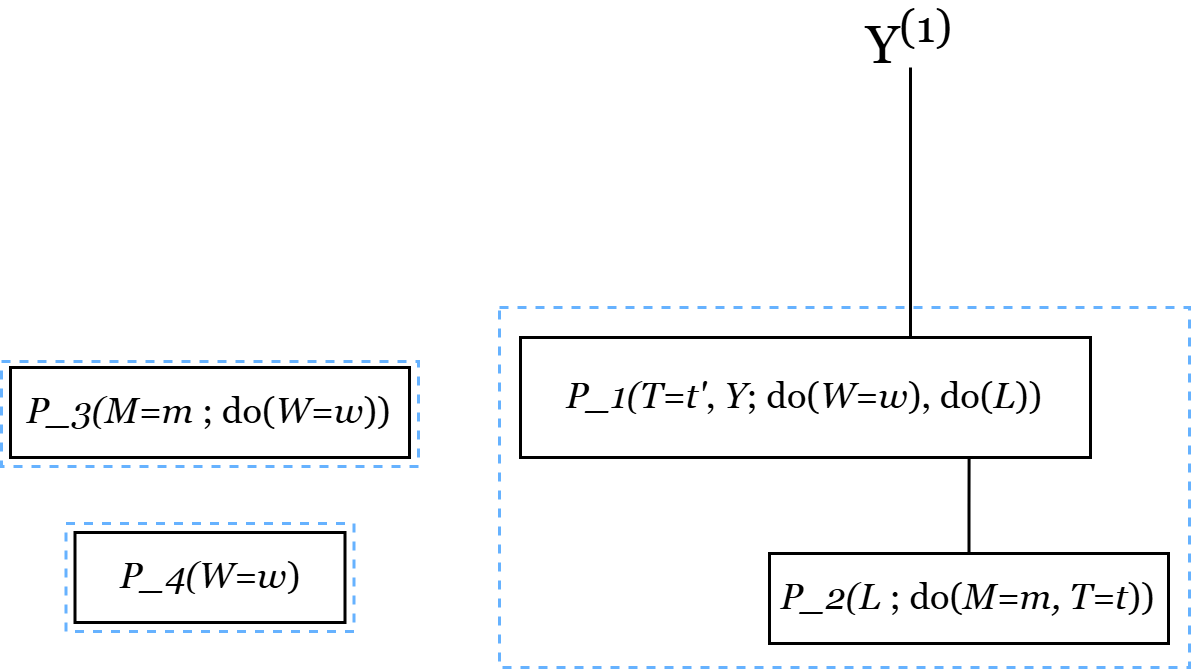
\includegraphics[width=\textwidth]{idcf.png}
\caption{Identified probability-box expression.}
\label{fig:re-expr}
\end{subfigure}

\caption{Running example (commute model $W,T,M,L,Y$), carried through the whole pipeline. (a)~the input ADMG and its rootification, replacing the bidirected edge $T\leftrightarrow Y$ by a shared latent root $R$; (b)~the parallel-world construction, where the factual outcome $Y$ and the counterfactual $Y_t$ remain coupled through $R$; (c)~the diagram after surgery and simplification; (d)~the identified estimand as probability boxes. Triangles are exogenous states, rounded boxes mechanisms, dots copy maps; blue dashed boxes mark normalisation.}
\label{fig:running-example}
\end{figure}

\paragraph{Comb-Disintegration Causal Inference Extension.}
In addition to counterfactual identification, the prototype includes a scoped causal-inference extension based on comb disintegration, exposed through \texttt{infer\_causal\_effect} rather than \texttt{identify\_counterfactual}. Given a Catlab string diagram, an observational joint distribution, and a user-specified comb structure (context, intervention, bridge, and outcome variables; the input contract is documented in the README API), it checks whether the diagram admits the required comb decomposition and, if so, computes the interventional effect $P(C \mid A, \mathrm{do}(X))$ numerically from the joint table.

This extension is demonstrated on a small smoking example and a larger HEPAR2-based clinical example---for instance, how chronic hepatitis would be distributed under interventions on hospital, surgery, and choledocholithotomy history, with injections and transfusion as bridge variables. Here the diagram serves only to validate that comb disintegration applies, while the numbers come from a separate finite synthetic joint table over the selected variables; lifting this limitation---attaching a stochastic map to each box and composing them to derive the joint directly---is left to future work.

\paragraph{Data Structures and Design Decisions.}
The data types track the pipeline stages above. Causal models are described by an \texttt{ADMGModel} (directed and bidirected edge lists), which Step~1's rootification turns into a \texttt{ConfoundedModel} (directed edges plus a map from each latent root to the variables it confounds); a \texttt{CounterfactualQuery} specifies, per world, the interventions, observations, and output variables. From simplification onwards every state is a Catlab \texttt{WiringDiagram}, so identification proceeds entirely by pattern-matching on box names and rewiring, with no separate symbolic graph representation. Final expressions use a small term language (atomic probability factors, products, sums, fractions): identifiable queries are reported as algebraic formulas matching the output style of existing tools, and non-identifiable ones report the stage and box at which absorption failed.

Two further properties characterise the design. Because every intermediate stage is kept explicit and exported to Chyp, each transformation is inspectable---unlike symbolic tools, where decomposition and simplification are internal. And because the stages mirror the theoretical algorithm one-to-one, each can be tested and optimised independently; the \texttt{test/} suite exercises every stage as a separate module-level test set (the breakdown is listed in the README).

\section{Empirical Evaluation}\label{sec:discussion}
We evaluate the prototype along two dimensions. Correctness is assessed through a differential testing harness against \texttt{cfid}~\cite{cfid_package}, the reference R implementation of ID-CF on ADMGs; runtime is then measured against both \texttt{cfid} and the Python \texttt{y0} library. The harness first checks that we return verdicts consistent with an established tool, and the benchmarks measure the cost of obtaining them.

\paragraph{Differential correctness testing.}
The harness (in \texttt{comparisons/correctness/}) generates counterfactual identification problems, translates each case into both the Julia and the R \texttt{cfid} input formats, and compares the ID/FAIL verdicts returned by the two tools.

The corpus contains structured benchmark cases and randomly sampled bow-free ADMGs over 5--8 nodes. Each random graph is paired with a generated conditional counterfactual query, and cases that reduce to ordinary single-world interventional queries are filtered out. The comparison uses \texttt{cfid} version 0.1.9 and the interventional-data setting, matching the current scope of the implementation.

Across all $1860$ comparable cases (with no tool errors), the Julia implementation agrees with \texttt{cfid} on $1832$, a $98.5\%$ agreement rate. The few remaining boundary cases, where one tool returns ID and the other FAIL, do not necessarily indicate a defect: a FAIL can reflect a conservative limitation of an implementation rather than a proof of non-identifiability, so these are treated as targets for further investigation rather than counterexamples to soundness.



\paragraph{Runtime benchmarking.}
Given this high cross-tool agreement, we next compare runtime against \texttt{cfid} and \texttt{y0}. The harnesses live in \texttt{comparisons/\allowbreak runtime/} (\texttt{julia\_\allowbreak benchmark.jl}, \texttt{r\_cfid\_\allowbreak benchmark.R}, \texttt{python\_y0\_\allowbreak benchmark.py}); all timings are warm medians over repeated executions on a standard desktop. We use two families of inputs: three standard queries---\texttt{drug}, \texttt{party}, and a conditional counterfactual query on the real-world \texttt{hepar2} network---and synthetic graph families of controllable size and topology (\texttt{chain}, \texttt{fanin}, \texttt{dense}, and a confounded chain \texttt{chain\_bi} carrying bidirected edges). The warm-median runtimes are collected below for the standard queries (top block) and the synthetic families at $n=32$ (bottom block); each speedup ratio is the baseline total runtime divided by Julia's, so a value above $1$ means Julia is faster and below $1$ slower.

\begin{center}
\resizebox{\textwidth}{!}{%
\begin{tabular}{lrrrrr}
\toprule
Case & Julia (ms) & R \texttt{cfid} (ms) & Python \texttt{y0} (ms) & R/Julia & \texttt{y0}/Julia \\
\midrule
\texttt{drug}
    & $19.85$  & $53.37$   & $13.33$   & $2.69\times$ & $0.67\times$ \\

\texttt{party}
    & $10.15$  & $28.31$   & $4.84$    & $2.79\times$ & $0.48\times$ \\

\texttt{hepar2\_conditional}
    & $90.84$  & $7812.44$ & $2005.27$ & $86.00\times$ & $22.08\times$ \\
\midrule
\texttt{chain} ($n{=}32$)
    & $113.38$ & $694.98$  & $540.64$  & $6.13\times$ & $4.77\times$ \\

\texttt{fanin} ($n{=}32$)
    & $188.52$ & $714.90$  & $199.77$  & $3.79\times$ & $1.06\times$ \\

\texttt{dense} ($n{=}32$)
    & $302.95$ & $708.91$  & $474.46$  & $2.34\times$ & $1.57\times$ \\

\texttt{chain\_bi} ($n{=}32$)
    & $454.37$ & $170.59$  & $17.89$   & $0.38\times$ & $0.04\times$ \\
\bottomrule
\end{tabular}%
}
\end{center}

On the standard benchmarks (top block), the categorical tool is consistently faster than R \texttt{cfid}---by roughly $2.7\times$ on the small \texttt{drug} and \texttt{party} queries and by $86\times$ on the larger \texttt{hepar2\_conditional} network. The comparison with Python \texttt{y0} is more mixed: \texttt{y0} is faster on the small queries, where a direct graph-level implementation has lower overhead, but on \texttt{hepar2\_conditional} Julia is about $22\times$ faster, so the explicit simplification pipeline becomes more beneficial as the model grows.

A stage-level breakdown explains this. The dominant cost in the Julia pipeline is the explicit \emph{simplification} stage (in \texttt{drug} it accounts for most of the runtime), while identification itself (Steps~4--5) is lightweight; R \texttt{cfid}, by contrast, exposes the main computation through a single \texttt{identifiable} call. The categorical method thus trades a heavier simplification phase for a very light identification phase, which pays off when simplification substantially reduces the later problem, especially on larger or structurally favourable graphs.

The synthetic families expose this structure-dependence more clearly (bottom block). Julia is faster than R \texttt{cfid} on \texttt{chain}, \texttt{fanin}, and \texttt{dense}, and faster than \texttt{y0} on \texttt{chain} and \texttt{dense} (roughly comparable on \texttt{fanin}), so the diagrammatic pipeline is competitive on sparse and moderately connected structures. The result reverses only on the heavily confounded \texttt{chain\_bi} family, where Julia is slower than both baselines: bidirected confounding greatly inflates the cost of simplification, and this preprocessing---not identification, which stays small---dominates the total runtime.


\paragraph{Comb-Disintegration Causal Inference Benchmarks.}
We also evaluate the comb-disintegration extension against pyAgrum's \texttt{causalImpact}. This comparison is separate from the ID-CF one above: \texttt{cfid} and \texttt{y0} return symbolic identification formulas, whereas the comb-disintegration extension returns concrete numerical interventional distributions. We use HEPAR2-derived examples whose selected variables form clinically meaningful exposure-outcome patterns, running both tools on the same variables and comparing the resulting distributions.

Grouping the cases by selected comb size and taking the median warm-median runtime per group (the speedup is pyAgrum runtime divided by Julia's) gives:

\begin{center}
\setlength{\tabcolsep}{8pt}
\begin{tabular}{ccrrr}
\toprule
Group & Comb size & Julia (ms) & pyAgrum (ms) & pyAgrum/Julia \\
\midrule
$1$ & $3$ & $3.29$ & $2.60$ & $0.79\times$ \\
$2$ & $4$ & $3.82$ & $4.02$ & $1.05\times$ \\
$3$ & $5$ & $4.56$ & $6.55$ & $1.44\times$ \\
$4$ & $6$ & $7.15$ & $13.67$ & $1.91\times$ \\
$5$ & $7$ & $8.11$ & $16.75$ & $2.06\times$ \\
\bottomrule
\end{tabular}
\end{center}

\section{Discussion}\label{sec:conclusion}

We have presented a prototype for counterfactual identification on Bayesian networks built directly on the categorical semantics of string-diagram surgery, realising the full ID-CF pipeline as rewrites on Catlab wiring diagrams with a Chyp trace exported at every stage. The evaluation shows this is not merely feasible but competitive: the tool reproduces \texttt{cfid}'s results and is substantially faster on sparse and moderately dense models, at the cost of an explicit simplification phase that becomes the bottleneck on densely confounded graphs.

The current implementation has four main limitations, each pointing to a direction for future work.
\begin{itemize}
    \item \textbf{Scope:} the tool targets the ID-CF setting for discrete graphical models, resting on the usual causal-model assumptions (causal sufficiency, correct specification), and does not yet cover causal discovery or continuous latent-variable models; the bidirected-edge abstraction may also miss some hidden dependencies. A natural next step is to broaden the query class and integrate with probabilistic inference engines.
    \item \textbf{Structure-dependent performance:} the simplification stage relies on repeated full-graph traversals and dominates runtime, so on dense and especially bidirected-confounded graphs (e.g.\ \texttt{chain\_bi}) this preprocessing cost can erase or reverse the identification speedup. Incremental rewriting and more efficient wiring-diagram data structures would remove these repeated scans.
    \item \textbf{Visualisation:} Chyp export aids inspection but supports a limited character set (unsupported symbols are mangled in labels, most acutely in identification outputs) and does not scale to large diagrams; a dedicated interactive string-diagram visualiser, supporting splicing, intervention, and rewrite operations, would address this.
    \item \textbf{Verification and interoperability:} the explicit intermediate diagrams make every rewrite step inspectable, but the steps are not yet formally verified and there are no native integrations with other toolchains. Future work includes formal verification and integration with richer categorical and probabilistic toolchains---for example EfProb~\cite{cho2017efprob}---and connections to causal representation learning and reinforcement-learning pipelines.
\end{itemize}


\bibliographystyle{splncs04}
\bibliography{references}

\end{document}
